\section{Analysis}\label{sec:popmethod}

As said in Section 3, we will follow the Performance Optimization and Productivity\cite{popMethod} methodology. The POP Efficiency metrics are the base of the methodology. First, we usually run the application many times in a \textit{strong scaling} manner. Strong scaling means leaving the problem's size constant and increasing the resources, for example, running the same Alya input set with 1, 2, 4 and Nodes. Then we gather necessary data for computing the efficiency metrics from the previous runs. Once we have the metrics, we possess insight into the factors limiting the code's performance when scaling in the number of resources. From this insight, we can locate the zones in the code responsible for it and try to propose a better implementation.

\subsection{Efficiency metrics}

Pop efficiency metrics try to describe the sources of inefficiency. Figure 1 shows the representation of the metrics. The main feature of the metrics is that they are hierarchic. The hierarchy follows a multiplicative scheme. Multiplicative means that the multiplication of the children of a metric computes its value.

\begin{figure}[htbp]
\centering
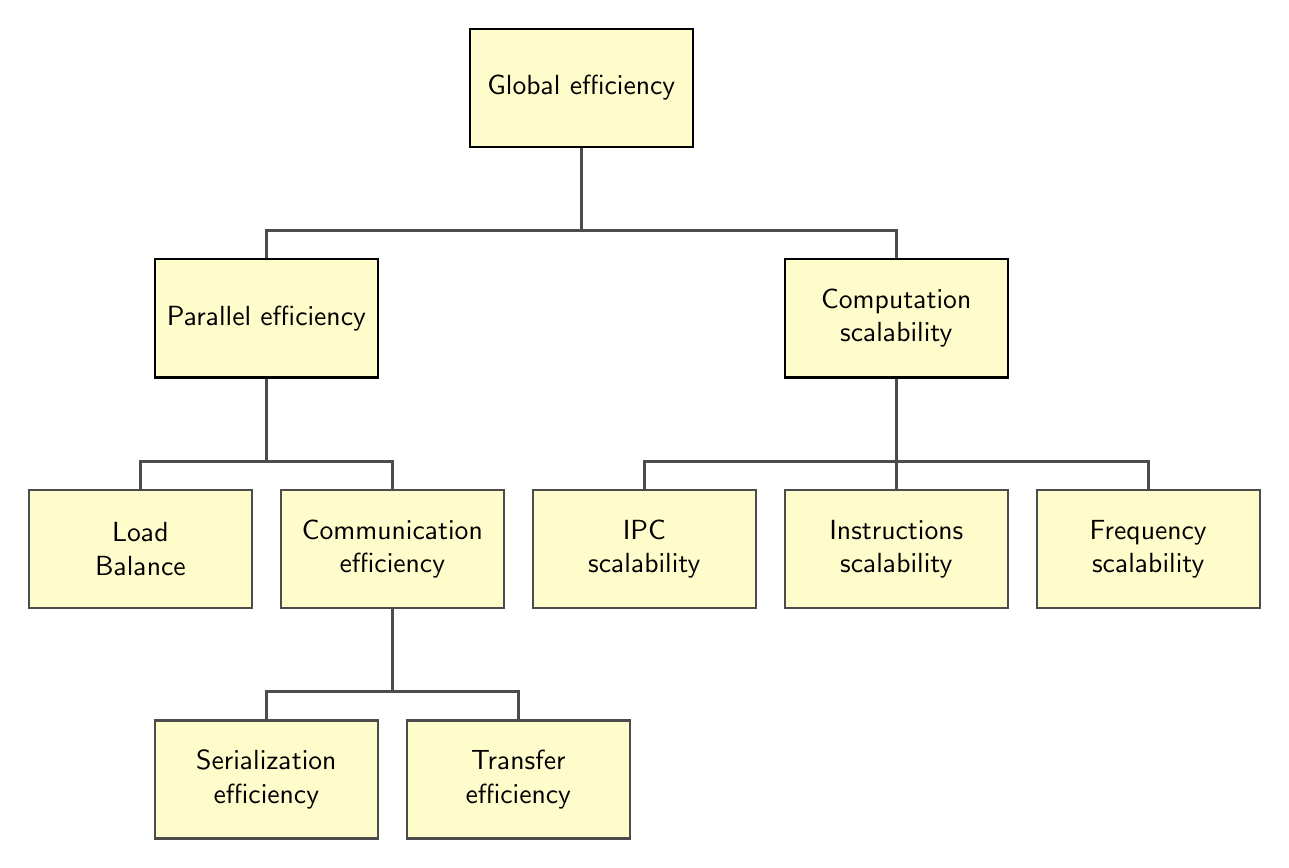
\begin{tikzpicture}[
% Label style
    label distance=3mm,
    every label/.style={blue},
% Event style
    event/.style={rectangle,thick,draw,fill=yellow!20,text width=2.6cm, minimum height=1.5cm,
		text centered,font=\sffamily,anchor=north},
% Children and edges style
    edge from parent/.style={very thick,draw=black!70},
    edge from parent path={(\tikzparentnode.south) -- ++(0,-1.05cm)
			-| (\tikzchildnode.north)},
    level 1/.style={sibling distance=8cm,level distance=1.4cm,
			growth parent anchor=south,nodes=event},
    level 2/.style={sibling distance=3.2cm},
    level 3/.style={sibling distance=3.2cm},
    level 4/.style={sibling distance=1cm}
%%  For compatability with PGF CVS add the absolute option:
%   absolute
    ]

  \node (glob) [event] {Global efficiency}
    child{node (par) {Parallel efficiency}
      child {node (lb) {Load  \\ Balance}}
      child {node (comm) {Communication efficiency}
        child {node (ser) {Serialization efficiency}}
        child {node (trans) {Transfer efficiency}}
      }
    }
    child{node (comp) {Computation scalability}
      child{node (ipc) {IPC \\ scalability}}
      child{node (ins) {Instructions scalability}}
      child{node (fre) {Frequency scalability}}
    };
\end{tikzpicture}
\caption[POP Efficiency metrics.]{POP Efficiency metrics. Own compilation.}
\label{popmet}
\end{figure}

The global efficiency describes how good is the application performance in general. Then, the global efficiency is represented by:

\begin{itemize}
  \item \textbf{Parallel efficiency:} Shows the efficiency lost due to splitting the work between processes and the effects of adding communications.
  \item \textbf{Computation scalability:} Represents the efficiency lost in useful computation. When we study a parallel application we look for computation side effects of the parallelization. For example, dividing the data among processes adds more instructions, running with more processes in the same machine can lower the IPC because of the resource sharing.
\end{itemize}

\subsubsection{Parallel efficiency}
\label{pareff}

Before entering in-depth on the metrics, we need to explain a few assumptions. 
The efficiency metrics estimate that each process can be in two states:
\begin{itemize}
  \item Useful state means that the process is performing computation. We usually represent a process in useful with the colour blue.
  \item Not useful state means that the process does not perform computation, such as sending an MPI message or waiting in a synchronization. We usually represent a process that is not useful with the colour red.
\end{itemize}

Figure \ref{fig:usefulnot} shows the graphical representation in a timeline of processes and their states. The x-axis represents the time, y-axis processes, and the colour of a process means the state that the process is in that time. The Figure shows four processes following the pattern: All computing, processes 3, 2 and 1 finish early and wait for process 0, then process 0 finishes and re-establish the computation.

    \begin{figure}[htbp]
      \centering
      \begin{tracedraw}{0.6}
        \tracedrawAddToLegend(\large{Not-useful}, red)
        \tracedrawAddToLegend(\large{Useful}, blue)
        \tracedrawEnableLineName(\large{Process})
        \tracedrawSetLegendColorScale(0.5)

        \tracedrawSetLineHeight(0.7)
        \tracedrawAddChunk[color=gray, fill=blue](94)
        \tracedrawAddChunk[color=gray, fill=red](3)
        \tracedrawAddChunk[color=gray, fill=blue](3)

        \tracedrawNewLine

        \tracedrawAddChunk[color=gray, fill=blue](50)
        \tracedrawAddChunk[color=gray, fill=red](47)
        \tracedrawAddChunk[color=gray, fill=blue](3)

        \tracedrawNewLine
        
        \tracedrawAddChunk[color=gray, fill=blue](45)
        \tracedrawAddChunk[color=gray, fill=red](52)
        \tracedrawAddChunk[color=gray, fill=blue](3)

        \tracedrawNewLine
        
        \tracedrawAddChunk[color=gray, fill=blue](30)
        \tracedrawAddChunk[color=gray, fill=red](67)
        \tracedrawAddChunk[color=gray, fill=blue](3)

      \end{tracedraw}
      \caption[Example of useful and not useful states.]{Example of useful and not useful states. Own compilation}
      \label{fig:usefulnot}
    \end{figure}

    We define $E$ as the total execution time, $P = \{p_1,p_2,\dots, p_n\}$ as the set of processes and for each process the set of time intervals where the process is in useful $U_p = \{u_1^{p},u_2^{p},\dots,u_{|U|}^{p}\}$ and the same set but when the process is in not-useful $\overline{U}_p$. Equation \ref{eq:timeuseful} shows the definition of $T_{U_p}$ which is the total time the process is in useful. Graphically expressed the sum of the blue chunks. The time the process is in not-useful $T_{\overline{U}_p}$ is defined similarly.

    \begin{equation}\label{eq:timeuseful}
      T_{U_p}=\sum_{U_p}\textcolor{blue}{\blacksquare}=\sum_{i=1}^{|U_p|}u^p_{i} 
    \end{equation}

    The parallel efficiency ($PE$) represents the time lost due to the parallelization. Then we can express it as the factor of the total time in useful by the total CPU time consumed. As we said, as the metrics are multiplicative it can also be computed with the product of the Load Balance ($LB$) and the Communication Efficiency ($CE$). Equation \ref{eq:PE} shows the formalization.

    \begin{equation}\label{eq:PE}
      PE=\frac{\sum_{i=1}^{|P|} T_{U_i}}{E\ast|P|}=LB\ast CE
    \end{equation}

    The Load Balance measures the efficiency lost due to improper work distribution. Expressed mathematically the factor between the average time in useful by the maximum time in useful. Equation \ref{eq:LB} shows the formalization.

    \begin{equation}\label{eq:LB}
      LB=\frac{\sum_{i=1}^{|P|}T_{U_{i}}}{|P|\ast max^{|P|}_{i=1}T_{U_i}}
    \end{equation}

    The Communication Efficiency measures efficiency lost due to spending time in not-useful state, namely, communications. Equation \ref{eq:CE} defines the CE. Expressed in words, is the maximum time in useful, divided by the total runtime. Also the Communication Efficiency is the multiplication of it's children, the Serialization Efficiency (SE) and Transfer Efficiency (TE).

    \begin{equation}\label{eq:CE}
      CE=\frac{max^{|P|}_{i=1} T_{U_i}}{E} = TE \ast SE
    \end{equation}

    As we said, the metrics are multiplicative. Therefore we can check that $PE=LB\ast CE$.
    Equation \ref{eq:checkPE} shows the check, we can see that the expression of efficiency lost by distributing improperly the work by the time lost in communications, expresses the Parallel Efficiency.

    \begin{equation}\label{eq:checkPE}
      LB \ast CE = \frac{\sum_{i=1}^{|P|}T_{U_{i}}}{|P|\ast max^{|P|}_{i=1}T_{U_i}} \ast \frac{max^{|P|}_{i=1} T_{U_i}}{E} = \frac{\sum_{i=1}^{|P|} T_{U_i}}{E\ast|P|} = PE
    \end{equation}

    As said, the Communication Efficiency can be expressed in terms of the Transfer Efficiency and the Serialization Efficiency.
    
    The Serialization Efficiency measures time lost in communications where there is not data to send or receive. Therefore, for calculating the metric we need to simulate an ideal network so no time because of transferring data is taken into account. Then the Serialization efficiency is the maximum computation time on an ideal network divided by the total runtime on an ideal network. Equation \ref{eq:SE} shows the expression where the suffix ideal means the time is on an ideal network.

    \begin{equation}\label{eq:SE}
      SE=\frac{max_{i=1}^{|P|}( T_{Uideal_{i}})}{E_{ideal}}
    \end{equation}

    The Transfer Efficiency measure time lost in not-useful due to data transfer. This can be computed with the factor of the runtime on ideal network by the runtime. Equation \ref{eq:TE} shows the mathematical expression.

    \begin{equation}\label{eq:TE}
      TE=\frac{E_{ideal}}{E}
    \end{equation}
    
    As done with the parallel efficiency, we can do the same check with the communication efficiency. Equation \ref{eq:checkCE} shows the check. We can see that the communication efficiency is represented by time lost due to the network not being ideal, which may seem it is not a thing we can not improve, but packing communications can solve it. And also time lost in not-useful without sending/receiving data.

    \begin{equation}\label{eq:checkCE}
      SE\ast TE=\frac{max_{i=1}^{|P|}( T_{Uideal_{i}})}{E_{ideal}} \ast \frac{E_{ideal}}{E} = \frac{max^{|P|}_{i=1} T_{U_i}}{E} = CE
    \end{equation}

\subsubsection{Computation scalability}

In the previous Section \ref{pareff} we have been discussing about efficiency. In this section we present the Computation Scalability, which this metric and its children refer to scalability, not efficiency.

This difference is important because the numbers depend on the baseline case. The Computation Scalability in strong scaling is defined as the ratio of the sum of all the useful computation time by the number of processes divided by the baseline ratio.

The factors that affect directly the computation scalability are:
\begin{itemize}
  \item \textbf{Instruction scalability:} Measures if the number of instructions scales with the number of processors. For example in strong scaling, if we double the number of processors, the ideal number of instructions executed should be the same. More instructions could mean that we are repeating work, or adding overhead from the parallelization.

  \item \textbf{IPC scalability:} Measures how the IPC evolves from the baseline, when we increase the number of processors on a run we can expect that the IPC is lower since the resources are shared with more processors. 

  \item \textbf{Frequency scalability:} Measures how the frequency evolves from the baseline, frequency of the processors should remain stable but pre-emptions and other side effects from running the application can affect the frequency and lower the performance.
\end{itemize}

Equation \ref{eq:texe} shows the execution time formula. We can observe that the execution time strictly depends on the computation scalability children.

\begin{equation}\label{eq:texe}
  T_{exe}=\frac{N_{ins}}{IPC\ast f}
\end{equation}

\subsection{Computing the efficiency metrics.}

Now that we understand the efficiency metrics that explain the performance of the code, we need to know how to apply it in practice. All the data we need for computing the efficiency metrics is:
\begin{itemize}
  \item Elapsed time.
  \item Maximum time in useful.
  \item Total time in useful.
  \item Elapsed time running in an ideal network.
  \item Average IPC in useful.
  \item Number of instructions executed in useful.
  \item Average frequency in useful.
\end{itemize}

\noindent
Fortunately the Barcelona Supercomputing Center has a set of tools that allow us to gather the data, automatize the extraction and calculating the Efficiency Metrics. The process consists of:
\begin{enumerate}
  \item Run the application with different number of processes with Extrae enabled.
  \item Select a focus of analysis, this consists of the relevant part of the code that we want to study. Usually the program initialization and finalization is not taken into account, and if the application uses an iterative pattern, we usually choose to focus on a set of iterations that represents the average iteration to study.
  \item Once we have the focus of analysis and the traces, we have to chop the traces so they just have the data of the focus of analysis.
  \item Finally we pass the chopped traces to the BasicAnalysis BSC tool which automatically extracts the data (including simulating the run with an ideal network using Dimemas) and computes the metrics. 
\end{enumerate}

The next sections bellow include a basic background on how to use the BSC tools for extracting the data for the Efficiency Metrics.

\subsubsection{Extrae}\label{extrae}

Extrae\cite{extrae} is a set of tools concerned to generate traces of executions for post-mortem analysis. There exist multiple ways for Extrae to intercept the program execution and get information. As we will be working with MPI we will use the \texttt{LD\_PRELOAD} method with intercepts the MPI calls and dumps the information.

For using this method we need:
\begin{itemize}
  \item A valid \texttt{extrae.xml} file including the different tracing options we want. 
  \item Choose the correct dynamic library to preload according to the programming model we are using. In our use-case we will use the pure MPI dynamic library. 
\end{itemize}

\noindent
Listing \ref{jobtrace} shows the integration of extrae with SLURM running an application \texttt{"BINARY"}. We add the call to \texttt{mpi2prv} tool because we disable automatic merging in the \texttt{extrae.xml} configuration file because we detected sometimes the tracing is stalled with the option enabled.

\begin{lstlisting}[language=sh, caption={Running a binary with SLURM and Extrae.}, label={jobtrace}]
#!/bin/bash
#SBATCH --job-name=alya-trace
#SBATCH --output=alya.out
#SBATCH --ntasks=48
#SBATCH --cpus-per-task=1
#SBATCH --time=1:20:00
#SBATCH --exclusive

export EXTRAE_HOME=#path to extrae installation
export EXTRAE_CONFIG_FILE=#path to extrae.xml

EXEC="env LD_PRELOAD=${EXTRAE_HOME}/lib/libmpitracef.so BINARY"
mpirun -np ${SLURM_NTASKS} ${EXEC}
$EXTRAE_HOME/bin/mpi2prv -f TRACE.mpits -o Alya-trace.prv -no-keep-mpits
\end{lstlisting}

\subsubsection{Paraver}

Paraver\cite{paraverPaper} is a visual inspection tool for analysis of parallel applications. The data the application needs is a trace in format \texttt{.prv} which are Extrae traces. This tool let us visually inspect the execution of applications. Therefore we can visually detect the pattern of the application, usually and in our use-case iterative and chop the trace having in the focus of analysis.

% TODO Tutorial?

\subsubsection{Dimemas}

Dimemas\cite{dimemas} is a command-line tool that given an input trace of an execution allows to remake the trace changing some conditions, for example, simulating an ideal network or changing some of the computational resources conditions. We will not enter in depth on how to use Dimemas as it is automatically called by BasicAnalysis (Section \ref{basicanalysis}).

\subsubsection{BasicAnalysis}\label{basicanalysis}

BasicAnalysis\cite{basic_analysis} is a suite of tools for,  as the name says, performing a basic analysis. We will focus just on the \texttt{modelfactors.py} tool.

The \texttt{modelfactors.py} tool automatically extracts and computes all the data needed for computing the POP metrics. We just need our set of chopped traces for a set of processes $P$. Listing \ref{modelfactorslst} shows how to run the tool inside a job script.

\begin{lstlisting}[language=sh, caption={Running modelfactors with SLURM.}, label={modelfactorslst}]
#!/bin/bash
#SBATCH --job-name=modelfactors
#SBATCH --output=modelfactors.out
#SBATCH --ntasks=1
#SBATCH --cpus-per-task=48
#SBATCH --time=1:20:00
#SBATCH --exclusive

modelfactors.py trace-48.chop1.prv trace-96.chop1.prv ...
\end{lstlisting}

\clearpage
Running it will output a table with the metrics computed and will output the following files:
\begin{itemize}
  \item \textbf{modelfactors.csv}: The POP metrics in a csv format.
  \item \textbf{modelfactors.gp}: A gnuplot\footnote{gnuplot site: \url{http://www.gnuplot.info/}} script file that projects the efficiencies to a high number of processes. Figure \ref{mfscaling} shows an example plot given by modelfactors tool.
\end{itemize}

\begin{figure}[htbp!]
  \centering
  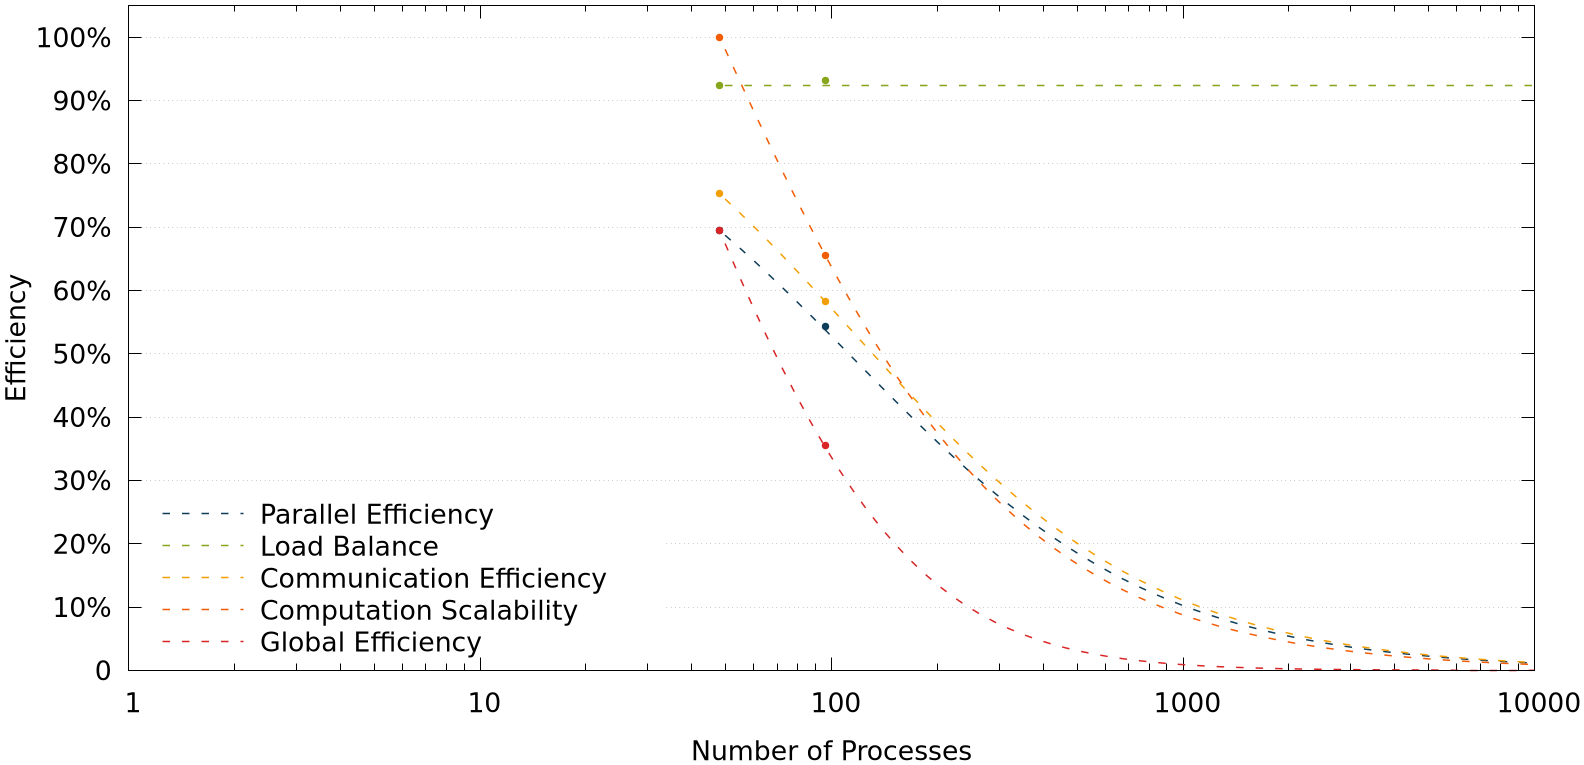
\includegraphics[width=0.8\textwidth]{modelfactorscale}
  \caption[Modelfactors projected efficiences.]{Modelfactors projected efficiencies. Own compilation.}
  \label{mfscaling}
\end{figure}

